\documentclass[12pt,compress,aspectratio=169]{beamer}
\input{../mybeamer}
\usepackage{pgfplots}
\pgfplotsset{compat=1.18}

\title{Class 14: Special Relativity}
\subtitle{Unit 5: Modern Physics}

\input{../term}
\input{../mycommands}
\newcommand{\bigsqrt}{\ensuremath\sqrt{1-\left(\dfrac vc\right)^2}}
\newcommand{\lorentz}{\ensuremath\frac1\bigsqrt}

\begin{document}

\begin{frame}
  \maketitle
\end{frame}



\section{Intro \& Review}

%\begin{frame}{What Everyone Knows}
%  
%  {\fontsize{60}{70}
%   \begin{displaymath}
%     \boxed{E=mc^2}
%   \end{displaymath}
%  }
%  
% \vspace{.2in} Most people know about \emph{this} equation, but what does it
% actually mean?
%\end{frame}



%begin{frame}{Review: Frame of Reference}
% A \textbf{frame of reference}\footnote{Or \textbf{reference frame}, or just
%   \textbf{frame}.} is the \emph{coordinate system} in which physical
% measurements are made. In \emph{classical} mechanics, a frame of reference is
% \begin{itemize}
% \item the $x$- $y$- and $z$-axes in the Cartesian coordinate system
% \end{itemize}
% \vspace{.2in}However, it may be more useful to think of the frame of
% reference as a ``hypothetical mobile laboratory'' an observer uses to make
% physical measurements (e.g.\ mass, lengths, time). At a minimum, it includes:
% \begin{itemize}
% \item A set of rulers (i.e.\ a coordinate system) to measure lengths
% \item A clock to measure the passage of time
% %\item A scale to compare forces
% %\item A balance to measure masses
% \end{itemize}
%end{frame}
%
%
%
%begin{frame}{Review: Frame of Reference}
% \begin{itemize}
% \item We assume that the ``hypothetical laboratory'' is \emph{perfect}
%   \begin{itemize}
%   \item The hypothetical ``instruments'' have zero errors
%   \item There are perfect instruments to measure anything you want
%   \end{itemize}
% \item What matters is the \emph{motion} (at rest, uniform motion, acceleration
%   etc) of your laboratory, and how it affects the measurement that you make
% \item ``From the point of view of\ldots''
% \end{itemize}
%end{frame}



\begin{frame}{Newtonian (Classical) Relativity}
  When we studied \emph{classical physics}\footnote{Also known as
    \emph{Newtonian} physics because of Newton's contribution}, we made some
  untested assumptions:
  \begin{itemize}
  \item\textbf{Absolute space:} \SI1{\metre} is \SI1{\metre} no matter where
    you are and how you are moving
  \item\textbf{Absolute time:} \SI1{\second} is \SI1{\second} no matter where
    you are and how you are moving
  \end{itemize}
  Under this assumption:
  \begin{itemize}
  \item Measurements of space and time are independent of motion of the
    observer
  \item\emph{All} velocities are relative to the frame of reference of the
    observer
  \item There is no such thing as \emph{absolute motion} or \emph{absolute rest}
  \item Motions of different frames of reference are related by the
    \textbf{Galilean velocity addition rule}:

    \eq{-.2in}{
      \vec v_{AC}=\vec v_{AB}+\vec v_{BC}
    }
  \end{itemize}
\end{frame}



\begin{frame}{Review: Inertial Frame of Reference}
  An \textbf{inertial frame of reference}\footnote{It is also known as a
  \textbf{rest frame} for obvious reasons} is a coordinate system that is
  moving in uniform motion (i.e.\ constant velocity, zero acceleration)
  \begin{itemize}  \item In an inertial frame, the laws of motion are valid
  \item %Since all uniform motions are equivalent,
    You may consider \emph{any} inertial frame to be \emph{at rest}
  \end{itemize}
  \vspace{.1in}
  \begin{center}
    \fcolorbox{black}{yellow!10}{
      \begin{minipage}{.85\linewidth}
        \textbf{The Principle of Relativity:} All laws of motion are equal in
        all inertial frames of reference.
      \end{minipage}
    }
  \end{center}
  The principle of relativity is a concept that is known to Galileo, and
  pre-dated Newton by several decades
\end{frame}



\begin{frame}{Example From Class 1: Inertial Frame of Reference}
  \begin{itemize}
  \item Observer A is moving uniformly with the skateboard relative to the
    road
    \begin{itemize}
    \item It is valid for A to think that he is at rest, but B is moving
    \end{itemize}
  \item Observer B is standing on the side of the road
    \begin{itemize}
    \item It is valid for B to think that he is at rest, but A is moving
    \end{itemize}
  \item A \& B observe different motion, but they agree on the \emph{physical
  law} (in this example, it is the kinematic equations)
  \end{itemize}
  \begin{center}
    \vspace{-.1in}
    \pic{.6}{graphics/57}
  \end{center}
\end{frame}





%\begin{frame}{New Physics: Maxwell's Equations}
%  \begin{columns}
%    \column{.2\textwidth}
%    \centering
%    \pic{1.2}{graphics/PORTRAIT-James-Clerk-Maxwell}\\
%    James Maxwell
%    
%    \column{.8\textwidth}
%    \begin{itemize}
%    \item For centuries, experimental results would always agree with this
%      ``Newtonian'' framework\ldots
%    \item By 1870s, instruments became accurate enough to measure behaviours
%      that were slightly different from prediction
%    \item \textbf{Maxwell's equations} in 1861 and 1862 are classical laws of
%      electrodynamics that explains the relationship between
%      \begin{itemize}
%      \item Electricity
%      \item Electric Circuits
%      \item Magnetism
%      \item Optics
%      \end{itemize}
%    \end{itemize}
%  \end{columns}
%\end{frame}



\begin{frame}{Maxwell's Equations}
  \textbf{Maxwell's equations} (introduced in Class 13) relate any disturbances
  in the electric and magnetic fields to the formation of a travelling
  \textbf{electromagnetic (EM) wave}\footnote{Also known as \textbf{EM
    radiation}, or just \textbf{radiation}}:

  \vspace{-.25in}{\large
    \begin{align*}
      \nabla\cdot\vec E &=\frac\rho{\varepsilon_0}\\
      \nabla\cdot\vec B &= 0\\
      \nabla\times\vec E &=-\frac{\partial\vec B}{\partial t}\\
      \nabla\times\vec B &=-\mu_0\vec J+
      \mu_0\varepsilon_0\frac{\partial\vec E}{\partial t}
    \end{align*}
  }
\end{frame}



\begin{frame}{Speed of Light}
  %Disturbances in electric \& magnetic fields propagate through space as
  %\textbf{electromagnetic (EM) waves}\footnote{Also known as \textbf{EM
  %  radiation}, or just \textbf{radiation}}.
  In a vacuum, Maxwell's equations predict that EM waves travel with a
  speed\footnote{Aptly called the \textbf{speed of light}} $c$ that is defined
  by two universal constants: the permittivity of free space ($\varepsilon_0$)
  and the permeability of free space ($\mu_0$):

  \eq{-.1in}{
    \boxed{
      c=\frac1{\sqrt{\varepsilon_0\mu_0}}=\SI{299792458}{\metre\per\second}
    }
  }

  The speed of any mechanical wave is defined relative to the medium in which
  it travels in. But what is the medium of an EM wave in a vacuum?
\end{frame}



%\begin{frame}{Peculiar Features of Maxwell's Equations}
%  \begin{itemize}
%  \item No mention of the \emph{medium} in which EM waves travels
%  \item When applying \emph{Galilean transformation} (classical equation for
%    relative motion), the law for magnetism breaks down: magnetic field lines
%    appear to have beginnings/ends
%  \item At first glance:
%    \begin{itemize}
%    \item In \emph{some} inertial frames, Maxwell's equations are simple and
%      elegant; but
%    \item In \emph{other} inertial frames (that are supposedly equal), they are
%      ugly and complex
%    \end{itemize}
%  \item Some physicists theorized that there may be a \emph{preferred} inertial
%    frame, which seems to violate the principle of relativity
%  \end{itemize}
%\end{frame}



\section{Michelson-Morley}

\begin{frame}{The Illusive Aether}
  Maxwell's hypothesis: $c$ is relative to a hypothetical \textbf{luminiferous
    aether}\footnote{For simplicity, we will just call it \textbf{ether}}. In
  order for ether to exist, it must have some fantastic\footnote{As in ``a
    fantasy'' that is too good to be true} properties:
  \begin{itemize}
  \item \emph{All} space is filled with ether
  \item Massless
  \item Zero viscosity
  \item Non-dispersive
  \item Incompressible
  \item Continuous at a very small (sub-atomic) scale
 \end{itemize}
  These properties makes ether (if it exists) very difficult to find
\end{frame}



\begin{frame}{The Michelson-Morley Experiment}
  If ether exists, at different times of the year, Earth should have different
  velocities relative to it. Ether would cause light to speed up, or slow down.
  \begin{center}
    \pic{.4}{graphics/2000px-AetherWind}
  \end{center}
  That is, if ether exists.
\end{frame}
  


\begin{frame}{The Michelson-Morley Experiment}
  German-American physicist Albert Michelson, an expert in light interference,
  designed an experiment to measure the effects of ether on the speed of light
  \begin{itemize}
  \item The experiment is ingenious but very difficult
  \item Used an ``interferometer'' designed by Michelson
  \item Later collaborated with American chemist Edward Morley
  \item Together performed the experiments over several years
  \end{itemize}
\end{frame}



%\begin{frame}{The Michelson Interferometer}
%  \pic1{graphics/michelsonmorley}\\
%\end{frame}



\begin{frame}{The Michelson Interferometer}
  \begin{columns}
    \column{.37\textwidth}
    \pic1{graphics/313754}

    \column{.63\textwidth}
    \begin{itemize}
    \item A beam of light is split into two using a two-way mirror
    \item The two beams are reflected and finally arriving at the screen
    \item The path are the same length; if the \emph{speed} of the light
      changes, we should see an interference pattern.
    \item\textbf{Except none were ever found!} (The interference pattern
      found was well below the predicted experimental error)
   \end{itemize}
  \end{columns}
\end{frame}



\begin{frame}{Dealing with ``Null Result''}
  The Michelson-Morley experiment failed to detect the ether, even after many
  refinements. What does this mean?
  \begin{itemize}
  \item Majority view:
    \begin{itemize}
    \item\textbf{The experiment was flawed!}
    \item Keep improving the experiment (or design a better experiment) and the
      ether will eventually be found
    \end{itemize}
  \item Minority view:
    \begin{itemize}
    \item\textbf{The hypothesis is wrong!}
    \item The experiment showed it for what it is: ether cannot be found
      because it's a bad hypothesis
    \end{itemize}
  \item A few physicists: there must be \emph{another explanation}
  \end{itemize}
\end{frame}



\begin{frame}{Hendrik Lorentz: Length Contraction}
  \begin{columns}
    \column{.2\textwidth}
    \centering
    \pic1{graphics/lorentz}\\    
    {\scriptsize Hendrik Antoon Lorentz\par}  

    \column{.8\textwidth}
    \begin{itemize}
    \item Considered the Michelson-Morley experiment to be significant
    \item Hypothesis: if objects travelling along the direction of ether
      contracts in length by a factor $\beta$
      
      \eq{-.1in}{
        \boxed{\beta=\bigsqrt}
      }

      \vspace{-.05in}the experimental results would be nullified
    \item No known physical phenomena can cause anything to contract without
      applying an enormous force
    \item Lorentz's equation is correct, but his approach was wrong
    \end{itemize}
  \end{columns}
\end{frame}



\begin{frame}{Poincar\'{e}: Time Dilation}
  French mathematician Henri Poincar\'{e} also hypothesized that ether affects
  the flow of time in the direction of motion. He derived an equation similar
  to Lorentz:

  \eq{-.1in}{
    \boxed{t'=\frac t{\bigsqrt}}
  }
 
  \begin{itemize}
  \item\vspace{-.1in}But \emph{no known physical phenomena} can alter the flow
    of time, just as no physical phenomena can compress an object without an
    external force
  \item Both Poincar\'{e} and Lorentz depended their hypothesis on
    \begin{itemize}
    \item Absolute time and space
    \item Existence of ether
    \end{itemize}
 \end{itemize}
\end{frame}



\section{Einstein}

\begin{frame}{Making Maxwell's Equations Work}{Albert Einstein in 1905, Age 26}
  \begin{columns}
    \column{.23\textwidth}
    \centering
    \pic1{graphics/Einstein_patentoffice}\\
    {\scriptsize Albert Einstein in 1905\par}
        
    \column{.75\textwidth}
    \begin{itemize}
    \item Einstein was working as a patent clerk in Switzerland
      \begin{itemize}
      \item Believed in the principle of relativity, and therefore
      \item Rejected the concept of a preferred frame of reference
      \end{itemize}
    \item In order to make Maxwell's equations to work again, Einstein
      revisited two of the most fundamental concepts in physics: \emph{space}
      and \emph{time}
    \end{itemize}
  \end{columns}
\end{frame}



\begin{frame}{Special Relativity}
  \vspace{.15in}Published in the journal \emph{Annalen der Physik} on September
  26, 1905 in the article ``\emph{On the Electrodynamics of Moving Bodies}''
  \begin{itemize}
  \item Submitted on June 30, 1905 and passed for publication
  \item Mentions 5 other scientists: Newton, Maxwell, Hertz, Doppler and Lorentz
    \begin{itemize}
    \item No references to any of their publications, and
    \item Provided no experimental results
    \end{itemize}
 %\item Initially ignored by most physicists, until Max Planck took interests
  \item It describes a ``special case'' without effects of gravity
  \item Later published the theory of ``general relativity'' in 1915 which
    included the effects of gravity (much more complicated)
  \end{itemize}
\end{frame}



\begin{frame}{Postulates of Special Relativity}
  In the journal article, Einstein posed two postulates:
  \begin{center}
    \fcolorbox{black}{yellow!10}{
      \begin{minipage}{.86\linewidth}
        \textbf{The Principle of Relativity:} All \emph{physical laws} are
        equal in all inertial frames of reference.
      \end{minipage}
    }
  \end{center}
  \begin{itemize}
  \item Reaffirms the principle in which \emph{all} physics is based on
  \item Extends the principle to include Maxwell's equations
  \end{itemize}
  \begin{center}
    \fcolorbox{black}{yellow!10}{
      \begin{minipage}{.86\linewidth}
        \textbf{The Principle of Invariant Light Speed:} Light always
        propagates in a vacuum with a definite velocity $c$, independent of the
        motion of the emitting body.
      \end{minipage}
    }
  \end{center}
  \begin{itemize}
  \item This is the logical interpretation of the first postulate
  \item The speed of light predicted in Maxwell's equations must apply to
    \emph{all} inertial frames of reference
  \end{itemize}
\end{frame}



\begin{frame}{Classical vs.\ Special Relativity}
  \textbf{Classical (Newtonian) relativity:}
  \begin{itemize}
  \item Space and time are \emph{absolute}, therefore
  \item The speed of light must \emph{always} be relative to the observer
  \item The speed of light from any light source depends on the motion of
    the source, and whether it is moving towards/away from the observer
  \end{itemize}
  \vspace{.2in}
  \textbf{Einstein says: This is impossible! This violates Maxwell's equations
    and the principle of relativity.}
\end{frame}



\begin{frame}{Special Relativity}
  \textbf{Special relativity:}
  \begin{itemize}
  \item Speed of light is absolute, therefore
  \item Space and time \emph{must} be relative
  \item We must modify our traditional concepts:
    \begin{itemize}
    \item Measurement of space (our ruler in the $x$-, $y$- and $z$-directions)
    \item Measurement of time (our clock)
    \item Concept of simultaneity (whether two events happens at the same time)
    \end{itemize}
  \end{itemize}
\end{frame}



\section{Simultaneity}

%\begin{frame}{Simultaneity: Thought Experiment}
%  If you see two sets of fire works ignite at exactly the same time--one off to
%  your left and the other far to your right. About $100m$ behind you, a car is
%  travelling along a highway at $95km/h$. Do the passengers in the car see the
%  fire works igniting simultaneously or do they think that one set ignited
%  before the other?
%\end{frame}


\begin{frame}{Relativity of Simultaneity: A Thought Experiment}
  Lightning bolts strike the two ends of a high-speed moving train.
  \begin{center}
    \vspace{-.1in}
    \pic{.42}{graphics/87-1-1024x673}
  \end{center}
  \vspace{-.25in}
  \begin{itemize}
  \item Two independent events: lightning striking the front, and lightning
    striking the back of the train
  \item The man on the ground sees the lightning bolt striking at the same time
  \item The woman on the train sees the lightning bolt on the front first
  \end{itemize}
\end{frame}



\begin{frame}{Relativity of Simultaneity: A Thought Experiment}
  From the man's perspective:
  \begin{itemize}
  \item He is stationary; the train and the woman are moving
  \item When the lightnings strike, he is at equal distance from the front
    and the back of the train
  \item The flash from the two lightning bolts arrive at his eyes at the same
    time
  \end{itemize}
 
  \vspace{.1in}Therefore, his conclusions are:
  \begin{itemize}
  \item The two lightnings must have occurred simultaneously
  \item The woman on the train was wrong: she \emph{thinks} that the lightning
    struck the front first because she's moving towards the light from the front
  \end{itemize}
\end{frame}



\begin{frame}{Relativity of Simultaneity: A Thought Experiment}
  Now, from the woman's perspective:
  \begin{itemize}
  \item\emph{She} and the train are stationary; the man and the world are moving
  \item When the lightnings strike, she is at equal distance from the front and
    back of the train
  \item The flash from the front arrive first, then the back
  \end{itemize}
  
  \vspace{.1in}Therefore, her conclusions are:
  \begin{itemize}
  \item Lightnings must have struck the front first
  \item The man on the road was wrong: he \emph{thinks} that
    the lightning struck at the same time because he's moving towards the light
    from the back
  \end{itemize}
\end{frame}



\begin{frame}{Relativity of Simultaneity: A Thought Experiment}
  \begin{itemize}
  \item The two observers disagree on the result, but
    \begin{itemize}
    \item Neither person is wrong
    \item Neither person is misinformed
    \end{itemize}
  \item Both observers are valid \emph{inertial} frames of reference
  \item This means that simultaneity depends on your motion
  \end{itemize}
  
  \vspace{.2in}\textbf{Events that are simultaneous in one inertial frame of
    reference are not simultaneous in another.}
\end{frame}



\section{Time Dilation}

\begin{frame}{Relativity of Time: Time Dilation}
  \begin{center}
    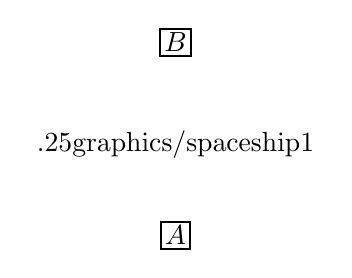
\begin{tikzpicture}
      \node at (0,0) {\pic{.25}{graphics/spaceship1}};
      \node[thick,draw=black,inner sep=1.5pt] at (0,1.3) {$B$};
      \node[thick,draw=black,inner sep=1.5pt] at (0,-1.15) {$A$};
    \end{tikzpicture}
  \end{center}
  \vspace{-.15in}I'm on a spaceship travelling in deep space, and I shine a
  light from $A$ to $B$. The distance between $A$ and $B$ is:
  
  \eq{-.23in}{
    |AB|=ct
 }

  \vspace{-.15in}I know the speed of light $c$, and I know how long it took
  ($t$) for the light pulse to reach $B$.\footnote{For convenience, we will use
  $t$ instead of $\Delta t$ for time interval in this class.}
\end{frame}



\begin{frame}{Relativity of Time: Time Dilation}
  \begin{center}
    \begin{tikzpicture}
      \node at (0,0) {\pic{.55}{graphics/spaceship2}};
      \node[thick,draw=black,inner sep=1.5pt] at (-2.4,2) {$B$};
      \node[thick,draw=black,inner sep=1.5pt] at (-2.4,-.2) {$A$};

      \node[thick,draw=black,inner sep=1.5pt] at (.2,2) {$B'$};
      \node[thick,draw=black,inner sep=1.5pt] at (.2,-.2) {$A'$};

      \node[thick,draw=black,inner sep=1.5pt] at (2.8,2) {$B''$};
      \node[thick,draw=black,inner sep=1.5pt] at (2.8,-.2) {$A''$};

      \draw[vectors,red] (-1,2.5)--(1,2.5) node[right]{$v$};
    \end{tikzpicture}
  \end{center}
  You are on a small planet watching my spaceship go past you at speed $v$. You
  see that same beam of light travel from $A$ to $B'$ instead.
\end{frame}



\begin{frame}{Relativity of Time: Time Dilation}
  We can relate the time interval measured by me on the spaceship ($t$) and
  your time interval on the planet ($t'$) using Pythagorean theorem:
  \begin{columns}
    \column{.3\textwidth}
    \begin{tikzpicture}[vectors,red]
      \draw (0,0)--(0,2)
      node[pos=0, below left,black]{$A$}
      node[midway,left,black]{$ct$}
      node[left,black] {$B$};
      \draw (0,2)--(4,2)
      node[midway,above,black]{$vt'$}
      node[right,black]{$B'$};
      \draw (0,0)--(4,2) node[midway,below, black]{$ct'$};
    \end{tikzpicture}
   
    \column{.7\textwidth}
    \begin{align*}
      (ct')^2 &=(vt')^2 + (ct)^2\\
      \left(c^2-v^2\right)t'^2 &=c^2t^2\\
      \left(1-\frac{v^2}{c^2}\right)t'^2 &=t^2\quad\rightarrow\quad
      \boxed{t'=\frac t\bigsqrt}
    \end{align*}
  \end{columns}
  
  \vspace{.2in}\textbf{Relativity of time}: the passage of time as measured by
  two observers in two different inertial references are different
\end{frame}



\begin{frame}{Relativity of Time: Time Dilation}
  The passage of time as measured by two observers in two different inertial
  frames of reference are related by:
  
  \eq{-.1in}{
    \boxed{t'=\frac t\bigsqrt}
  }
  \begin{center}
    \begin{tabular}{l|c|c}
      \rowcolor{pink}
      \textbf{Variable} & \textbf{Symbol} & \textbf{SI Unit}\\ \hline
      Proper time (ordinary time)  & $t$  & \si\second \\
      Dilated time (expanded time) & $t'$ & \si\second \\
      Speed               & $v$ & \si{\metre\per\second}\\
      Speed of light      & $c$ & \si{\metre\per\second}
    \end{tabular}
  \end{center}
  \begin{itemize}    
  \item\textbf{Proper time} is measured by an observer \emph{at rest} relative
    to the events
  \item\textbf{Dilated time} is measured by a \emph{moving} observer in another
    inertial frame
  \end{itemize}
\end{frame}



%\begin{frame}{Relativity of Time: Time Dilation}
%  \eq{0in}{
%    \boxed{t' =\frac t{\bigsqrt}}
%  }
%  \item Since $\bigsqrt < 1$, $\Delta t > \Delta t_0$.
%  \end{itemize}
%\end{frame}



\begin{frame}{A Very Insightful Example Problem}
  \textbf{Example:} A rocket speeds past an asteroid at $0.800c$. If an
  observer in the rocket sees \SI{10.0}{\second} pass on her clock, how long
  would that time interval be as seen by an observer on the asteroid?

  \uncover<2->{
    \vspace{.3in}\textbf{Example:} A rocket speeds past an asteroid at
    $0.800c$. If an observer in the \emph{asteroid} sees \SI{10.0}{\second} pass
    on his clock, how long would that time interval be as seen by an observer
    on the \emph{rocket}?
  }

  \uncover<3->{
    \vspace{.3in}How can that be?
  }
\end{frame}



\section{Length Contraction}

\begin{frame}{Relativity of Space: Length Contraction}
  Captain Quick is a comic book hero who can run at nearly the speed of light.
  In his hand, he is carrying a bomb with a lit fuse set to explode in
  \SI{1.50}{\micro\second}. The bomb must be placed into its bracket before
  this happens. The distance ($L$) between the bomb and the bracket is
  \SI{402}\metre.
\end{frame}


\begin{frame}{Relativity of Space: Length Contraction}
  \begin{center}
    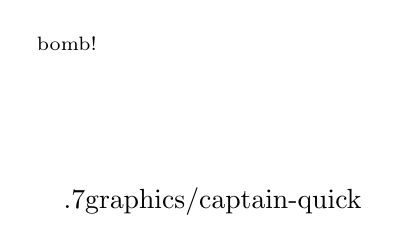
\begin{tikzpicture}
      \node at (0,0) {\pic{.7}{graphics/captain-quick}};
      \node[fill=white] at (-1.85,2) {\scriptsize bomb!};
      \end{tikzpicture}
  \end{center}
  Both Captain Quick and the observers on the side of the road agree that
  he is moving at $v=\SI{2.00e8}{\metre\per\second}$ relative to the bracket.
\end{frame}



\begin{frame}{Relativity of Space: Length Contraction}
  If Captain Quick runs at \SI{2.00e8}{\metre\per\second}, according to
  classical mechanics, he does not make it in time, and the bomb will explode:
  \begin{displaymath}
    t=\frac Lv=\frac{402}{\num{2.00e8}}
    =\SI{2.01e-6}\second=\SI{2.01}{\micro\second}
  \end{displaymath}
  In fact, this is the amount of time that the observer on the side of the road
  measures.
\end{frame}



\begin{frame}{Relativity of Space: Length Contraction}
  To the observer at the side of the road, the time on the bomb is slowed due
  to time dilation. A time interval of $t'=\SI{2.01}{\micro\second}$ for the
  side of the road is, in fact:
  \begin{align*}
    t' = \frac t\bigsqrt\quad\rightarrow\quad t &= t'\bigsqrt
    = \num{2.01e-6}\sqrt{1-\left(\frac{2.00}{3.00}\right)^2}\\
    &= \boxed{\SI{1.50e-6}\second}
  \end{align*}
  The observer on the side of the road sees a passage of (dilated) time of
  $t'=\SI{2.01}{\micro\second}$, but Captain Quick, who is in the same
  reference frame as the bomb, experiences a passage of (proper) time of
  $t=\SI{1.50}{\micro\second}$, just before it explodes.
\end{frame}



\begin{frame}{Relativity of Space: Length Contraction}
  If Captain Quick sees only $t=\SI{1.50}{\micro\second}$, then how \emph{far}
  did he travel? From his frame of reference, the distance he travels is
  contracted by the same factor as time dilation, i.e:
 
  \eq{-.1in}{
    \boxed{L'=L\bigsqrt}
  }

  For this example, Caption Quick only travels \SI{300}{\metre} from his frame
  of reference:
  \begin{displaymath}
    L'=L\bigsqrt=402\sqrt{1-\left(\frac23\right)^2} = \boxed{\SI{300}\metre}
  \end{displaymath}
\end{frame}



\begin{frame}{Relativity of Space: Length Contraction}
  Length contraction only occurs in the direction of motion
  \begin{center}
    \pic{.8}{graphics/baseball-contraction}
  \end{center}
\end{frame}



\begin{frame}{Lorentz Factor}
  The \textbf{Lorentz factor} $\gamma$ is a short-hand for writing length
  contraction, time dilation and relativistic mass:
  
  \eq{-.1in}{
    \boxed{\gamma=\lorentz}
  }
  Then time dilation and length contraction can be written simply as:
  
  \eq{-.1in}{
    \boxed{\Delta t'=\gamma \Delta t}\quad\quad\boxed{L'=\frac L\gamma}
  }
\end{frame}



\begin{frame}{Example Problem}
  \textbf{Example:} A spacecraft passes Earth at a speed of
  \SI{2.00e8}{\metre\per\second}. If observers on Earth measure the length of
  the spacecraft to be \SI{554}\metre, how long would it be according to its
  passengers?
\end{frame}



\section{Relative Motion}

\begin{frame}{Let's Summarize}
  \begin{center}
    \begin{tikzpicture}[scale=2,vectors]
      \draw (1,.5)--(2,.5) node[pos=0,left]{\textbf{A}};
      \draw (3,0)--(2,0) node[pos=0,right]{\textbf{B}};
    \end{tikzpicture}
  \end{center}
  If A and B are moving uniformly with respect to one another (doesn't matter
  if they're moving towards, or away from each other)
  \begin{itemize}
  \item They do not agree whether any events happens at the same time or not
  \item Each sees the other's clock running slow
  \item Each sees the other ``contracted'' in length along the direction of
    motion
  \end{itemize}
\end{frame}



\begin{frame}{Relative Velocities}
  The Galilean velocity addition rule violates the postulates of relativity, so
  Einstein replaces it with \textbf{Einstein velocity addition rule}:
  
  \eq{-.1in}{
    \boxed{v_{AC}=\frac{v_{AB}+v_{BC}}{1+\dfrac{v_{AB}v_{BC}}{c^2}}}
  }

  When velocities are slow ($v_{AB}\leq c$, and $v_{BC}\leq c$) we recover the
  Galilean velocity addition rule.
\end{frame}



%\begin{frame}{But What About\ldots}
%  We've studied the most important principles in special relativity already,
%  but what about:
%
%  \vspace{-.2in}{\Huge
%    \begin{displaymath}
%      \boxed{E=mc^2}
%    \end{displaymath}
%  }
%
%  We seem to be no closer to learning about it!
%\end{frame}



\section{Momentum \& Mass}

\begin{frame}{Relativistic Momentum}
  Recall that momentum is mass times velocity (displacement over time). But
  since displacement $\Delta\vec x$ and time $t$ both depend on the motion, we
  need modify the expression for \emph{relativistic} motion to get the
  expression for \textbf{relativistic momentum}:
 
  \eq{-.1in}{
    \boxed{
      p=\frac{m\vec v}\bigsqrt
    }
  }
  
  (We have not changed the \emph{definition} of momentum, only the underlying
  assumptions about space and time when calculating momentum.)
\end{frame}




\begin{frame}{Relativistic Mass}
  Relativistic momentum shows that mass is also relativistic:
  The \textbf{apparent mass}\footnote{also known as \textbf{relativistic mass}}
  ($m'$) as measured by a moving observer is related to its
  \textbf{rest mass}\footnote{also known as \textbf{intrinsic mass} or
    \textbf{invariant mass}} ($m$) by:

  \eq{-.13in}{
    \boxed{m'=\frac m\bigsqrt=\gamma m}
  }
  \begin{center}
    \begin{tabular}{l|c|c}
      \rowcolor{pink}
      \textbf{Variable} & \textbf{Symbol} & \textbf{SI Unit}\\ \hline
      Relativistic mass (measured in moving frame) & $m'$ & \si{\kilo\gram}\\
      Rest mass (measured in stationary frame) & $m$  & \si{\kilo\gram}\\
      Speed               & $v$ & \si{\metre\per\second}\\
      Speed of light      & $c$ & \si{\metre\per\second}\\
      Lorentz Factor      & $\gamma$ & (no unit)
    \end{tabular}
  \end{center}
  %As an object speeds up, it will behave as if it is more massive. As
  %$v\rightarrow c$, $m\rightarrow\infty$.
\end{frame}



\begin{frame}{Example Problem}
  \textbf{Example:} An electron has a rest mass of \SI{9.11e-31}{\kilo\gram}.
  In a detector, it behaves as if it has a mass of \SI{12.55e-31}{\kilo\gram}.
  How fast is that electron moving relative to the detector?
\end{frame}



\section{Mass-Energy Equivalence}

\begin{frame}{Force and Work}
  Recall that force is the rate of change in momentum:

  \eq{-.1in}{
    \vec F=\frac{\Delta\vec p}{\Delta t}%=\frac{d\vec p}{dt}
  }

  and work is force times displacement:

  \eq{-.1in}{
    W=\int\vec F\cdot d\vec x=\Delta K
  }

  We can substitute the impulse expression for force, then substitute expression
  for relativistic momentum, and after some calculus\ldots
\end{frame}



\begin{frame}{Work and Kinetic Energy}

  \eq{-.2in}{
    W=\frac{mc^2}{\bigsqrt}-mc^2 = \Delta K
  }

  From the work-energy theorem, the work $W$ done by a force $\vec F$ is equal
  to the change in kinetic energy, $\Delta K$
\end{frame}



\begin{frame}{Relativistic Energy}
  From the work-energy theorem, we obtain the expression for relativistic
  kinetic energy:
  
  \eq{-.1in}{
    \boxed{K=m'c^2-mc^2}
  }
  \begin{center}
    \begin{tabular}{l|c|c}
      \rowcolor{pink}
      \textbf{Variable} & \textbf{Symbol} & \textbf{SI Unit}\\ \hline
      Kinetic energy of an object & $K$  & \si\joule \\
      Relativistic mass (measured in moving frame) & $m'$ & \si{\kilo\gram}\\
      Rest mass (measured in stationary frame) & $m$ & \si{\kilo\gram}\\
      Speed of light                           & $c$ & \si{\metre\per\second}
    \end{tabular}
  \end{center}
\end{frame}



\begin{frame}{Relativistic Energy}%{What This All Means}

  \eq{0in}{
    \boxed{K=m'c^2-mc^2}
    %\boxed{K=m'c^2-mc^2=(\gamma-1)mc^2}
  }

  \vspace{-.1in}The minimal energy that any object has, regardless of it's
  motion (or the lack of motion) is its \textbf{rest energy}:
  
  \eq{-.2in}{
    E_0=mc^2
  }
  
  \vspace{-.13in}The \textbf{total energy} of an object has is
   
  \eq{-.2in}{
    E_T=m'c^2=\gamma mc^2
  }

  \vspace{-.1in}The difference between total energy and rest energy is the
  kinetic energy:
  
  \eq{-.2in}{
    K=E_T-E_0=(\gamma-1)mc^2
  }
\end{frame}



\begin{frame}{Mass-Energy Equivalence}%{What This All Means}
 
  \eq{0in}{
    \boxed{E=mc^2}
  }
  \begin{itemize}
  \item\vspace{-.2in}Whenever there is a change of energy, there is also a
    change of mass
  \item Two conservation laws in classical physics:
    \begin{itemize}
    \item Conservation of mass
    \item Conservation of energy
    \end{itemize}
    must be combined into a single \textbf{conservation of mass-energy}
  \item Mass-energy equivalence doesn't just mean that mass can be converted
    into energy and vice versa\footnote{This is absolutely true, as you have
    already seen in discussion on nuclear physics in Physics 11}, but rather,
    one can be converted into the other \emph{because they are fundamentally
    equivalent}
  \end{itemize}
\end{frame}



%begin{frame}{A General Rule for Scientific Discoveries}
% When a physicist ``discovers'' a new physical law, it is not enough that the
% new law explains what could not be explained before, but it also has to be
% consistent with what is already explained.
%
% \vspace{.2in}In the case of kinetic energy, that means that Einstein's
% relativistic equation must agree with Newtonian (classical) mechanics for
% $v\leq c$
%end{frame}
%
%
%
%begin{frame}{Kinetic Energy: Classical vs.\ Relativistic}
% \begin{columns}
%   \column[t]{.5\textwidth}
%   \textbf{Relativistic:}
%
%   \eq{-.1in}{
%     K=\frac{mc^2}{\bigsqrt}-mc^2%\left(\lorentz-1\right)mc^2
%   }
%   
%   \column[t]{.5\textwidth}
%   \textbf{Newtonian:}
%
%   \eq{-.1in}{
%     K=\frac12mv^2
%   }
% \end{columns}
% Are they different? If we do a binomial series expansion of the square-root
% term, we get:
%
% \eq{-.1in}{
%   K = mc^2
%   \left(1+\frac12\frac{v^2}{c^2}+\cdots\right) -
%   mc^2 \approx\frac12mv^2+\cdots
% }
%
% when $v\ll c$, we recover the $\dfrac12mv^2$ expression that we know so well!
%end{frame}



\begin{frame}{Comparing Classical and Relativistic Energy}
  \begin{columns}
    \column{.53\textwidth}
    In classical mechanics, kinetic energy $K$ is a quadratic function of
    speed $v$:

    \eq{-.1in}{
      K=\frac12mv^2
    }
   
    In relativistic mechanics, $K\rightarrow\infty$ as $v\rightarrow\infty$
    with an asymptote at $v=c$:
    
    \eq{-.1in}{
      K=m'c^2-mc^2
    }

    \column{.42\textwidth}
    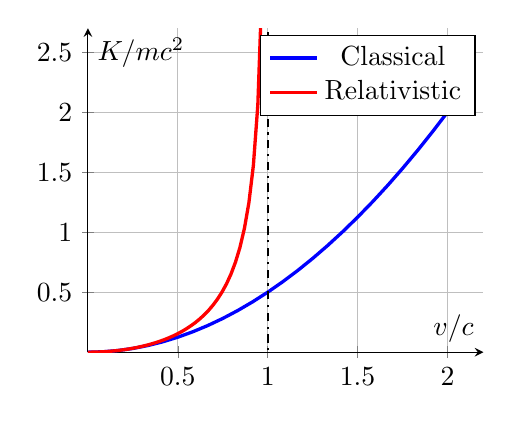
\begin{tikzpicture}
      \begin{axis}[
          axis lines = center,
          grid = both,
          width=2.6in,
          xmin=0,xmax=2.2, xlabel={$v/c$},
          ymin=0,ymax=2.7, ylabel={$K/mc^2$},
          ytick={0,.5,...,3}
        ]
        \addplot[blue,very thick,domain=0:2]{1/2*x^2};
        \addlegendentry{Classical}

        \addplot[red,very thick,domain=0:.97,samples=40]{1/sqrt(1-x^2)-1};
        \addlegendentry{Relativistic}
        
        \addplot[thick,dash dot] coordinates{(1,-1)(1,4)};
      \end{axis}
    \end{tikzpicture}
  \end{columns}
  These two equations are in good agreement for $v<0.3c$. Only at
  higher speeds does relativistic effects have to be accounted for
\end{frame}



\begin{frame}{Example Problem}
  \textbf{Example:} A rocket car with a mass of \SI{2.00e3}{\kilo\gram} is
  accelerated from rest to \SI{1.00e8}{\metre\per\second}. Calculate its
  kinetic energy:
  \begin{enumerate}
  \item Using the classical equation
  \item Using the relativistic equation
  \end{enumerate}
\end{frame}
\end{document}
